\documentclass[12pt]{article} 
\usepackage{amsmath} 
\usepackage[dvips]{graphicx}
\usepackage{multirow} 
\usepackage{geometry} 
\usepackage{pdflscape}
\usepackage[labelfont=bf]{caption} 
\usepackage{setspace}
\usepackage[running]{lineno} 
% \usepackage[numbers,sort]{natbib}
\usepackage[round]{natbib} 
\usepackage{array}
\usepackage[table]{xcolor}
\usepackage{xr}

\newcommand{\methods}{\textit{Materials \& Methods}}
\newcommand{\SI}{\textit{Appendix}~}

\topmargin -1.5cm % 0.0cm 
\oddsidemargin 0.0cm % 0.2cm 
\textwidth 6.5in
\textheight 9.0in % 21cm
\footskip 1.0cm % 1.0cm

\usepackage{authblk}

\title{Do motif roles provide unique information about species risk of extinction?}

\author{Anna \r{A}kesson$^{1\dagger}$, Alyssa R. Cirtwill$^{3}$, Kate Wootton$^{2}$, Gyuri Barab\'{a}s$^{1}$, Anna Ekl\"{o}f$^{1}$} 
\date{\small$^1$Department of Theoretical Biology, Chemistry, and Physics\\ 
Link\"{o}ping University\\
Link\"{o}ping, Sweden\\
\medskip
\small$^2$ Swedish Agricultural University\\
Uppsala, Sweden\\
\medskip
\small$^3$Department of Agricultural Sciences\\
University of Helsinki\\
Helsinki, Finland\\
\medskip
$^\dagger$ Corresponding author:\\
}


\begin{document} 
\maketitle 
\raggedright

\setlength{\parindent}{15pt} 
\begin{spacing}{2.0}

% Maybe Proc B - approached Alyssa re: other motifs paper, flexible length limit (but pay extra over X pages).

% Try to reorder following a sensible discussion
% Mention chain, direct competition briefly and then get rid of them. 

\section*{Abstract}

    Bottom-up effects of disturbance to basal resources can strongly affect the persistence of consumers.
    However, predicting which species will be most affected by increasing levels of disturbance is not straightforward.
    In-degree and trophic level are known to affect a consumer's vulnerability to bottom-up disturbance, but these are relatively coarse measures of a species' place in its food web.
    Here we explore how roles based on participation in three-species motifs are related to persistence, and how these motif-based roles relate to simpler measures.
    We found that networks containing a higher proportion of the `omnivory' motif, where a predator consumes a prey and the prey of that prey, tend to have higher mean persistence following disturbance to basal species, and that more frequent participation in the omnivory motif was associated with higher probability of persistence.
    However, the relationship between omnivory and persistence was highly variable across networks; much more so than for the other motifs we consider.
    % % Something to wrap all of this up, including degree and TL.

    - can we condense omnivory, in-degree any further?
    - - at least omnivoryhttps://www.overleaf.com/project/602a809ce82587324badb832
    - can we shorten any more? Nice to save some money?
    - glossaryhttps://www.overleaf.com/project/602a809ce82587324badb832
    - refs
    - ending

    - Fig. 4 not much in discussion, could be a candidate for the SI? Or add more discussion about apparent competition, etc. in discussion sections per motif

\clearpage
\section*{Introduction}

    %\subsection*{1 Why are bottom-up effects important for understanding stability?}
     The plant community is the foundation upon which the myriad of species in terrestrial food webs depend for their survival \citep{}. Disturbances in the plant community have been shown to affect important ecosystem properties such as primary \citep{} and secondary production \citep{borer2012plant}, soil respiration and carbon cycling \citep{chen2019plant} and consumer diversity \citep{scherber2010bottom, Baiser2016}. The stability of the plant community is crucial for sustaining a healthy energy flow in the ecosystem as a whole \citep{Rosenblatt2016} and the structure of the plant community promotes stability across all different levels of ecosystem organization \citep{proulx2010diversity,scherber2010bottom}. Loss of diversity at the basal level typically causes declines in both abundance and richness of all types of consumers, e.g. herbivores, predators, and parasitoids \citep{scherber2010bottom}.
     %This has been shown in both theoretical work~\citep{} and empirical experiments ~\citep{} and results from the vertical propagation of disturbances through the network of interacting species.
    
     %\subsection*{2 Bayesian networks are a fantastic way to model bottom-up effects}
    The study of how an initial population decline or extinction leads to loss of other species via direct and indirect effects (i.e., secondary extinctions) is a vibrant area of research \citep{curtsdotter2011robustness, dunne2009cascading, Eklof2006}. Traditionally, there are two main approaches for studying secondary extinctions. First, there are topological models, which are solely based on food web structure \citep{dunne2009cascading}. Here, initial extinctions only affect other species in the network once a consumer has lost all of its prey and therefore must go extinct. The second approach uses dynamical models, which explicitly simulate population dynamics using a system of differential equations \citep{binzer2011susceptibility}. Dynamical models take changes in prey or predator densities into account when calculating the densities of other species in the network. These models therefore describe complex effects such as indirect interactions and are generally more realistic than topological models. However, dynamical models are parameter intensive, can only include a limited number of species, and simulations are time-consuming. 
    
    
    A middle‐ground approach for simulating secondary extinctions are Bayesian networks \citep{Eklof2013}. In this framework, a consumer's probability of extinction depends on the fraction of resources lost and on a baseline probability of extinction which captures causes unrelated to the network structure (e.g., disease, stochastic extinction of small populations). Modelling Bayesian networks is fast and computationally efficient, allowing analysis of networks with high species richness \citep{Haussler2020}. 
    As consumers do not affect the extinction probabilities of their resources, Bayesian networks can only capture bottom-up effects of disturbances within networks. However, Bayesian networks do capture the majority of secondary extinctions captured by dynamical models \citep{Eklof2013}.
    This emphasizes the importance of bottom-up effects in food webs and makes Bayesian networks the ideal framework to use when studying them.  

    %\subsection*{3 Global scale network properties are known to affect stability}
    The global structural properties of ecological networks have implications for their functioning \citep{Petchey2002}, stability \citep{Allesina2012} and robustness to disturbances \citep{Dunne2002d, Eklof2006}. For example, more highly-connected networks are more resistant to secondary extinctions \citep{Dunne2002d, Eklof2006} and a modular organization, where some groups of species are tightly interconnected with limited connections between groups, can limit the propagation of disturbances \citep{}.
    %\subsection*{4 meso-scale nw propoerties also affect stability}
    Structural properties on the local scale, i.e. properties of single species, are also well-studied and there is consensus that species with high trophic levels, few prey (low in-degree), and low abundances are generally at higher risks of secondary extinction \citep{binzer2011susceptibility}. However, in-degree and trophic level are both relatively coarse descriptions of a species' role within its food-web~\citep{Cirtwill2018FoodWebs}. 
    For example, specialists may not necessarily have a high risk of extinction if it consumes a basal resource which is at low risk of being affected of disturbance. On the other hand, a consumer with low trophic level may still be at high risk of extinction if it consumes preys which themselves possess high risk of being affected by disturbance. 
    
    
    %\subsection*{5 Motif participation may similarly affect species' particular extinction risk}
    One way to incorporate more nuance into descriptions of how species fit into their communities is to define species' roles based on their participation in different motifs -- unique combinations of small numbers of interacting species~\citep{Stouffer2007,Stouffer2012}. Importantly, these `motif roles' capture information about species' direct and indirect interactions, incorporating larger-scale network structure into species-level descriptions. 
    This means that two species with the same in-degrees and trophic levels can still participate in different sets of motifs if, for example, one interacts with specialists and the other interacts with generalists~\citep{Cirtwill2018FoodWebs}. 
    This extended description of species structural roles may give additional information of extinction risk or synthesize the information provided by multiple other measures of a species' place in its community.
    At the network level, the frequencies of different motifs are associated with community stability \citep{prill2005dynamic, bascompte2005simple} and with changes to the composition of plant communities~\cite{giling2019plant}. 
    We therefore expect that the motif structure of a network and species' participation in that structure should be related to risks due to disturbance to basal resources. 
    
           %\subsection*{Here we test...}
    Specifically, we are interested in whether a consumer's extinction risk depends on 1) the motif profile of the full food web and 2) the motifs in which a focal species participates. 
    In addition, we want to understand how the information provided by motifs is related to classical global and local food web properties in order to better integrate different aspects of network theory.
    Of the 13 three-species motifs that can occur in empirical food webs there are four motifs that are over-represented in empirical networks and are thought to contribute to stability \citep{Stouffer2007, Borrelli2015a, giling2019plant}: the three-species chain, omnivory, apparent competition and direct competition motifs.
    These four motifs are also the ones which can occur in the acyclic networks required for Bayesian network simulations~\citep{Eklof2013}. 
    Therefore, we focus on these four particularly important motifs.  
    

 
    
   % \subsection*{Other, simpler measures of species' roles can also affect extinction risk, and may correlate with motif participation}

    	%Species with high trophic levels may be more likely to go extinct since they depend upon the stability of relatively long food chains~\citep{}. 
        %For the same reasons, the number of motifs a species participates in will also tend to be larger in larger and more-connected networks.
    	%Likewise, the range of possible trophic levels increases with network size, although higher connectance may keep trophic levels low as long as the shortest food chain carries more weight (as in prey-averaged and shortest path trophic levels). 
        %A species' trophic level in turn may affects a species' motif role by restricting the set of positions in which it can appear~\cite{Cirtwill2018EcolLett}. 
    	%To unravel to what extent species motif roles gives additional information on species' probabilities of going extinct, we therefore need to take network structure and other role definitions into account.

    	
\section*{Methods}

	\subsection*{Initial network construction}

		We generated a realistic set of simulated networks based on the niche model~\citep{Williams2000,Stouffer2007} using the function "nichemodel" within the Julia~\citep{Julia} package \emph{BioEnergeticFoodWebs}~\citep{bioenergfw,Delmas2017}. 
		To capture a range of plausible network architectures, we simulated networks with sizes ranging from 50 to 100 species (in steps of 10) and connectances ranging from 0.02 to 0.18 (in steps of 0.04). 
		For full details, see~\citet{Cirtwill2021_inprep}.
        We then filtered these simulated networks to remove any with unreasonable structures.
		Specifically, we removed any network containing disconnected components (species or groups of species not connected to the rest of the network) or any network where the shortest path between a consumer and the closest basal resource was \textgreater6 (as these high trophic levels are very uncommon in empirical food webs ~\citep{}).
		New networks were simulated to replace any removed networks, and this process was repeated until we obtained 100 suitable networks in each combination of size and connectance.
              
		A Bayesian food web depicts probabilistic relationships among a set of species where each species' probability of persistence depends upon the probabilities of its resource species persisting~\citep{Jensen_Nielsen,Eklof2013}. 
		Therefore, all persistence calculations follow a strict bottom-up routine beginning by determining the status of the primary producers (who do not depend on other species) and continuing on to primary consumers (who depend only on primary producers), and so on up the network.
		
		While the niche-model food webs can contain cycles (e.g., species A eats B, B eats C, and C eats A), such cycles make it impossible to calculate persistence in the Bayesian network framework~\citep{Tarjan1972}. We therefore removed any cycles within each network.
		To render networks acyclic, we followed~\citet{Allesina2009} and broke cycles by removing links which do not contribute to the robustness of the food web.
		This is achieved by first finding the set of resources for each consumer and then removing the consumer-resource connections which have the lowest eigenvalue centrality~\citep{Allesina2009}.
		These links have the least effect on the overall stability of the network; removing them creates an acyclic network with very similar properties to the original network.
		Next, we order the species from lowest to highest trophic level using a topological sorting routine following \citep{Tarjan1972, Allesinaetal2005}, ensuring that probability calculations follow a strict bottom-up order. 
        After these steps, calculations of persistence probabilities can begin.

	\subsection*{Calculating persistence}	

		First, we assigned all species a baseline probability of extinction ($\pi_{base}$) -- the risk of going extinct given factors not related to the food web itself. 
		For consumer species, this also applies to extinction despite all resources being present. 
		Such events can, for example, reflect diseases or stochastic extinctions of small populations. 


		As well as this baseline scenario, we simulate a set of scenarios where primary producers get a higher baseline probability of extinction ($\pi_{disturbed}$). 
		These scenarios reflect threats to primary producers such as increased temperatures resulting in droughts, making some species more vulnerable to extinction.
		$\pi_{disturbed}$ ranged between $0.1-0.5$, in steps of $0.08$. The highest disturbance level, $\pi_{disturbed} = 0.5$, corresponds to basal species having a 50\% risk of going extinct. 
		Consumer species retained $\pi_{base}=0.1$ in all cases.
		
		
		As well as the intrinsic baseline probability of extinction, extinction risk for consumers is affected by access to resources. 
		When all resources are extant, the probability of extinction for a consumer $i$, $P(\lnot i)$, is equal to the baseline probability; $P(\lnot i|X_{1},...,X_{n}) = \pi_{base}$. 
		When all resources are extinct, the consumer will go extinct; $P(\lnot i|\lnot X_{1},...,\lnot X_{n})=1$. 

		Calculating $P(i)$ or $P(\lnot i)$ is less straightforward when a consumer $i$ loses a fraction $k/n = f$ of its prey. 
		Plausible ecological responses to losing some prey include i) a topological response, where the consumer's probability of extinction is constant unless all resources are lost, ii) a linear response, in which the extinction probability increases linearly with resources loss, and iii) several nonlinear responses where the probability of extinction increases non-linearly with the fraction resource lost. 
		The extinction probability will differ depending on the response function. 
		We use a sigmoid non-linear functional response of consumers to the loss of resources ($\alpha >1, \beta >1$) which has been shown to most accurately capture the secondary extinctions produced by a dynamical model~\citep{Eklof2013}. 
		We use a cumulative density function of a beta distribution for this purpose:
		\begin{equation}
		\label{betafunc}
		P(\lnot i|f) = \pi_{i} + (1 - \pi_{i}) \frac{B(f;\alpha,\beta)}{B(\alpha,\beta)}
		\end{equation}

		We calculate the fraction of resources lost ($f$) for each consumer $i$, to compute $P(\lnot i|f)$. 
		Persistence is determined by comparing $P(\lnot i|f)$ with a randomly drawn number from a uniform distribution between 0-1. 
		If this random number is lower than $P(\lnot i|f)$, the species is considered extinct. 
		The species' marginal probability of persistence is simply $P(i) = 1-P(\lnot i)$.
		In this manner we calculate persistence probabilities for all species in the network, starting from the bottom and working our way up. 
		Probabilities of extinction for resource species are used when calculating probabilities for higher level species. 
		Some species will be extinct due to primary extinctions (stochastic extinction with all resources left), while others will experience secondary extinctions; as a response to primary extinctions (partial or total loss of resources). 
		As this method is probabilistic, repeating the simulation will yield different results. 
		To minimize the effect of this variation we repeat these calculations 100 000 times per web, with unique random draws when calculating $P(i)$.
		The final persistence for each species is the mean over these runs. 

	\subsection*{Defining motif profiles and participation [species roles]}

        As a first measure of the meso-scale structure, we calculated the `motif profile' of each network.
        This is, in our case, a four-dimensional vector of the number of each three-species motif in the network.
        To separate differences in motif structure from differences in network size, we normalized motif profiles by dividing the count of each motif by the total count of all motifs.
        The motif profile for each network therefore describes the proportions of each motif and has a sum of exactly one.

    
        We then describe meso-scale structure at the species level by defining each species' motif participation and motif roles.
        Motif participation describes the frequency with which a focal species appears in each of the four motifs, analogous to the network motif profile~\citep{Stouffer2012}.
        A species' motif role describes the frequency with which a focal species appears in each \emph{unique position} (e.g., top, middle, or bottom species in the three-species chain, top or bottom species in the apparent competition motif) within each motif ~\citep{Stouffer2012,Cirtwill2017}.
		We calculated species' motif participation and roles using the Python package \emph{pymfinder}~\citep{pymfinder}.
        As with motif profiles of networks, we normalized participation (and role) vectors by dividing each count by the total number of motifs (motif positions) the species appears in.
        Note, however, that this normalization does \emph{not} control for differences due to degree \emph{per se} as high-degree species also tend to participate in different types of motifs than low-degree species~\citep{Cirtwill2021_inprep}.
        
        
        Finally, we calculated simpler measures of a species' role within its community: degree and trophic level.
		As the Bayesian network approach only accounts  bottom-up effects, out-degree (number of predators) is irrelevant to extinction risk.
		We therefore focused on species' in-degrees (number of prey).
		Note, however, that out-degree may also be important in topological simulations which include both top-down and bottom-up effects. 


		There are many definitions of trophic level available, most of which tend to be very similar~\citep{Carscallen2012}.
		Here we use shortest trophic level (STL): the length of the shortest food chain between the focal species and any basal resource~\citep{Williams2004}. 
		Basal resources have an STL of one, any species consuming a basal resource has an STL of two, etc.
        STL is therefore a measure of the minimum number of steps away a species is from any disturbance to the base of a food web.


	\subsection*{Statistical analysis} 

        \subsubsection*{How does network mean persistence vary depending on network properties?}
        
            Both species richness (S) and connectance (C) are known to influence persistence in both simulation studies and empirical food webs.
            In addition, increasing the probability of extinction for basal species ($\pi_{disturbed}$ above) is intended to decrease persistence of species at higher trophic levels.
            Although these effects are not the main focus of our manuscript, we must establish these background effects before measuring the effects of meso-scale structure on persistence.
            The persistence of basal species in our simulations is determined only by their baseline probability, being either $\pi_{base} = 0.1$ or higher, dependent on $\pi_{disturbed}$.
            We therefore considered only non-basal species (i.e., those with at least one prey) throughout this manuscript.

            To test for effects of global network properties, we fit a linear regression relating consumer species' probabilities of persistence to network size, connectance, the level of disturbance to basal resources, and all interactions between them. 
            All predictors were centered and scaled before fitting the model. 
            As the three-way interaction was significant, we did not simplify the model.
            All models were fit using the R~\citep{R} base function `lm'.

        
        \subsubsection*{How do network motif profiles vary with global structure?}
        
            As well as affecting persistence directly, global network structure (i.e., size and connectance) may affect the meso-scale structure of the network.
            This is especially likely since we include only networks which can retain all initial species after 1000 rounds of simulated Lotka-Volterra population dynamics~\citep{Cirtwill2021_inprep}:  some meso-scale structures might be more likely to allow all species to persist than others in networks with different size and connectance constraints.
            We test whether networks with the the same size and connectance have more similar motif profiles using a PERMANOVA~\citep{Anderson2001} of Bray-Curtis dissimilarity among motif profiles against network size, connectance, and their interaction.
            Significance was calculated based on 9999 permutations.
            PERMANOVA tests may give false positive results if variability is not homogeneous among groups (i.e., levels of network size or connectance).
            To test whether this applies in our case, we fit an ANOVA of the dispersion of motif profiles about the centroid for each combination of network size and connectance. 
            We fit the PERMANOVA using the function `adonis', calculated dispersion using the function `betadisper', and fit the ANOVA using the function `anova', all from the R~\citep{R} package \emph{vegan}~\citep{vegan}.
            To gain a more detailed picture of how the proportion of each motif may vary with global network structure, we also fit four regressions (one per motif) relating the proportion of a motif to network size, connectance, and their interaction.
            We fit each regression using the R~\citep{R} base function `lm'.
            
        
        \subsubsection*{How does network mean persistence vary with motif profiles?}

            To test whether networks with similar motif profiles tend to have similar mean persistences among consumers, we fit a PERMANOVA relating Bray-Curtis dissimilarity in motif profiles to the mean persistence of all consumers in a network (averaged across all levels of disturbance to basal resources).
            We then tested whether dispersion was homogeneous across levels of persistence using an ANOVA and whether there was a linear relationship between persistence (rounded to three decimal places) and variability of motif profiles using a linear regression.
            In case high or low mean persistences are associated with more variable network structure, we calculated dispersion of motif structure for each level of mean persistence (rounded to three decimal places to allow multiple networks to have the same value of mean consumer persistence and treated as a categorical variable). 
            All statistical tests were conducted as when relating motif profiles to global network structure.
            
            
            To supplement these overall tests, we also fit four regressions testing whether persistence had a linear relationship to the proportion of a network profile made up of each motif, and whether this varied with the level of disturbance.
            Each regression included the proportion of a motif, disturbance, and their interaction as predictors.
            All regressions were fit using the R~\citep{R} base function `lm'.
        
        
        \subsubsection*{How does species persistence vary with motif participation?}

            We are interested in whether participating more often in a certain motif (e.g., direct competition) might increase persistence.
            % (see \emph{Appendix SXX} for relationships between persistence and counts of motifs).
            To test this, we fit four linear mixed-effect models (LMMs; one per motif included in the Bayesian networks).
            These models included the proportion of the species' role made up by the focal motif, the level of disturbance to basal species, and the interaction between the two.
            We centered and scaled the predictors before fitting the LMMs.
            The models also included a random intercept for the interaction between species richness and connectance (equations.
            All models were fit using the R~\citep{R} function `lmer' from the package \emph{lmerTest}~\citep{lmerTest}.
            We calculated marginal (fixed effects only) and conditional (fixed and random effects) $R^2$ using the R~\citep{R} function `r.squaredGLMM' from the package \emph{MuMIn}~\citep{MuMIn}.

            The formula for these LMMs are:       
            
            \begin{equation}
                \Psi_{ik} \approx \rho_{i} + \pi_{disturbed_k} + \rho_{i}\pi_{disturbed_k} +
                S:C_{i} ,
                \label{propreq}
            \end{equation}


            where $\Psi_{ik}$ is the persistence of species $i$ during disturbance level $k$, $\rho_{i}$ is the proportion of the role of species $i$ that is made up by the focal motif, $\pi_{disturbed_k}$ is the probability of extinction for a basal resource in disturbance level $k$, and $S:C_{i}$ is a random intercept for the species richness and connectance of the network containing species $i$.
    
            We were also interested in whether these general trends were consistent across networks with different global properties and different levels of disturbance. 
            To test this, we performed a linear regression of persistence against motif participation within each simulated network, for each level of disturbance to basal resources.
            These regressions were fit using the R~\citep{R} base function `lm'.
            We then analyse the distribution of slopes for the effect of motif participation across levels of disturbance, network size, and connectance. 
            We performed similar analyses to test whether appearing in different positions in each motif (i.e., the motif role) is related to a species' persistence (\emph{Appendix SH}).

        \subsubsection*{How does persistence vary with degree and trophic level?}
        
            A species' motif participation is likely related to its in-degree and trophic level since all three properties are measures of network position.
            To provide context for the results above, we therefore fit two linear mixed-effects regressions relating persistence to degree or trophic level, $\pi_{disturbed}$, and their interaction.
            As above, we centered and scaled the predictors.
            We also included a random effect of the interaction between network size and connectance in order to account for the differences in persistence between different networks. 

        
        \subsubsection*{How does motif participation vary with species and network properties?}

            As with network profiles, species' motif participation may covary with other measures of network structure and species' roles within the network.
            To establish this context for motif participation, we fit a linear mixed-effect model relating the frequency of participation in each motif to network size, connectance, and their interaction, as for network motif profiles (\emph{Appendix SG}).
            We also fit linear mixed-effect models relating the count or proportion of each motif to degree or trophic level and a random effect of the interaction between network size and connectance using the R~\citep{R} function `lmer' from the package \emph{lmerTest}~\citep{lmerTest}.
            We performed similar analyses to test whether a species' motif role is related it in-degree or trophic level (\emph{Appendix SI}).


% % % Things in SI only
% persistence vs. motif positions - SH
% motif roles (positions) vs. other network properties - SI
% persistence vs. % Basal
% motif profiles vs. % Basal

\section*{Results}

    We were interested in i) how the distribution of motifs in a network (i.e., the network's \emph{motif profile}) affect network persistence, and ii) how a species motif participation affects its persistence. 
    We analysed this for different levels of disturbance to the basal level. 
    To provide context, we also investigated relationships between persistence and classic global (size and connectance) and local (in-degree and trophic level) network properties.

    
    \subsection*{Network mean persistence and global network properties}
    
        Increasing the probability of extinction for basal species necessarily decreased the mean probability of persistence for consumers. 
        This effect was clear across the ranges of network size and connectance we considered. 
        Network size and connectance also affected network mean persistence, but to a much smaller extent than increasing disturbance (Figure S1, Table S1, \emph{Appendix SA}). 
        Persistences generally decreased in more-connected networks, but the effect of network size varied depending on level of disturbance. 
        At low disturbance, small and highly-connected webs showed the lowest mean persistence, whereas at high disturbance, large and highly connected webs showed the lowest mean persistence (Fig. S2, \emph{Appendix SA}).

    \subsection*{Network motif profiles and global network properties}

        Although the PERMANOVA test relating overall motif profiles to network properties was not reliable (Fig. S3, \emph{Appendix SB}), 
        connectance was significantly related to the frequencies of different motifs in a network when considering motifs individually.
        Network size and the interaction between network size and connectance did not strongly affect the frequencies of most motifs (Fig.~\ref{motif_proportion_lms}).
        Considering each motif separately, the proportions of apparent competition and three-species chains in a network's motif profile tended to decrease with increasing connectance while the proportion of omnivory increased with increasing connectance (Table S2, \emph{Appendix SB}). 
    
        \begin{figure}[h!]
            \centering
            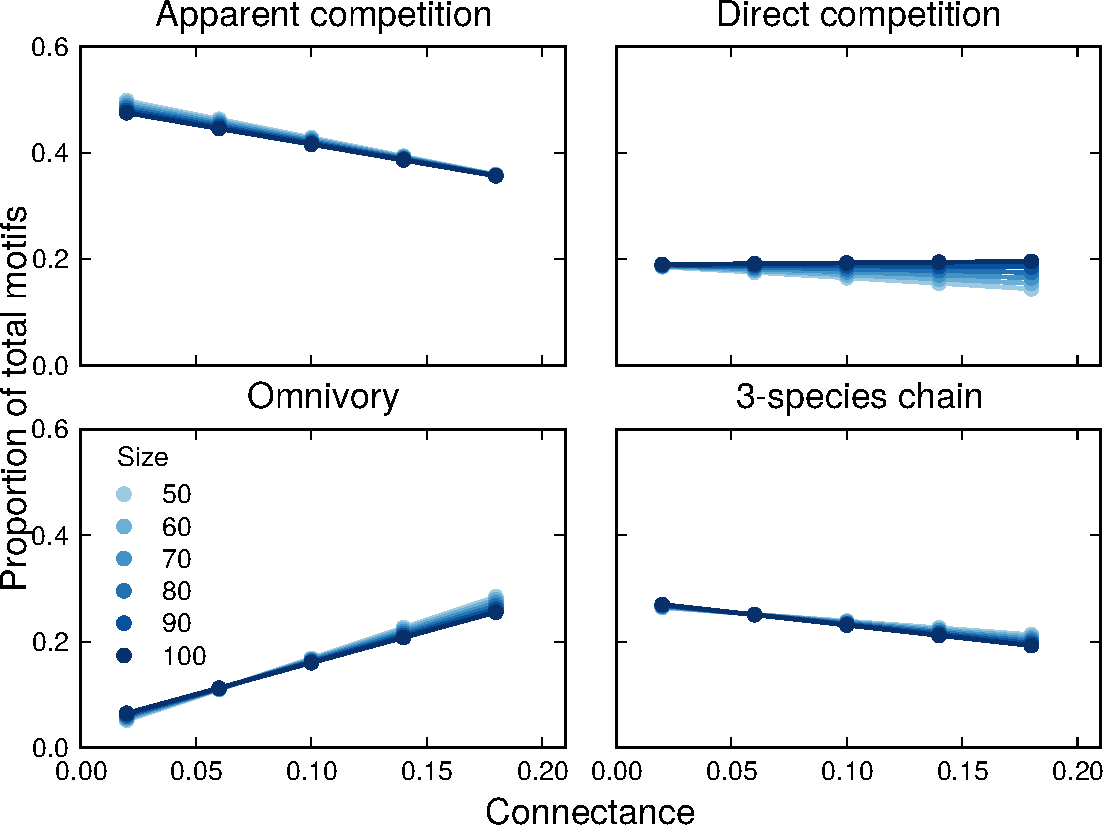
\includegraphics[width=.75\textwidth]{manuscript/figures/motif_proportion_lms.pdf}
            \caption{The proportions of a network's motif profile made up by the four motifs which can appear in acyclic networks varied with the size and connectance of the network. More-connected networks tended to contain relatively more omnivory motifs and fewer apparent competition motifs. The proportions of direct competition and three-species chain motifs were less variable.}
            \label{motif_proportion_lms}
        \end{figure}

    \subsection*{Network motif profiles and network mean persistence}
    
        The overall motif profile of a network was related to the average persistence of consumers ($F_{1,2998}$=571, $p$\textless0.001). 
        Average persistence was higher in networks with higher proportions of the chain, direct competition, and apparent competition motifs (Table S3, \emph{Appendix SC}). 
        Conversely, average persistence was lower in networks with higher proportions of the omnivory motif. 
        These trends were consistent across  levels of disturbance (Fig.~\ref{motif_profile_persistence}, Table S3), \emph{Appendix SC}).% Network persistence varies between networks with different dispersion of motif profiles ($F_{134,2865}$=2.19$\times10^{24}$, $p$=\textless0.001). For example, networks with more variable motif profiles have higher persistence ($\beta$=0.183, $p$\textless0.001).

        \begin{figure}
            \centering
            \includegraphics[width=.5\textwidth]{figures/persistence_motif_profiles.eps}
            \caption{The proportions of the four motifs in a network's motif profile were related to the mean persistence of species in the network. Specifically, persistence decreased as the proportion of omnivory in the network's motif profile increased while persistence increased with increasing proportions of the other three motifs. Interactions between motif profiles and disturbance were significant but small. Here we show the relationships of probabilities of extinction of basal resources of 0.1 (top set of lines) and 0.5 (bottom set of lines). Relationships are shown for the observed range of proportions for each motif.}      
            \label{fig:motif_profile_persistence}
        \end{figure}    

    \subsection*{Species motif participation and species persistence} 
    
       The relationship between frequency of participation in a motif and a species' probability of persistence depended on the level of disturbance. 
       When disturbance was low, species' persistence increased with increasing proportions of the omnivory and direct competition motifs. 
       Conversely, persistence decreased with an increasing proportion of the apparent competition motif. 
       Persistence was not significantly related to the proportion of the three-species chain motif (Figure~\ref{fig:prop_lmer_all}).
            
            
        At high levels of disturbance, a species' persistence decreased as the proportion of the three-species chain increased, but persistence increased as the proportion of any other motif increased (Figure~\ref{fig:prop_lmer_all}). 
        This means that increased disturbance strengthened the effects of the three-species chain motif and changed the direction of the effect of the apparent competition motif  (Table S4, \emph{Appendix SD}).
        The relationship between omnivory and persistence was still positive but weaker at higher levels of disturbance, and the relationship between persistence and direct competition was largely unaffected by disturbance.
    
            
            \begin{figure}[h!]
                \centering
                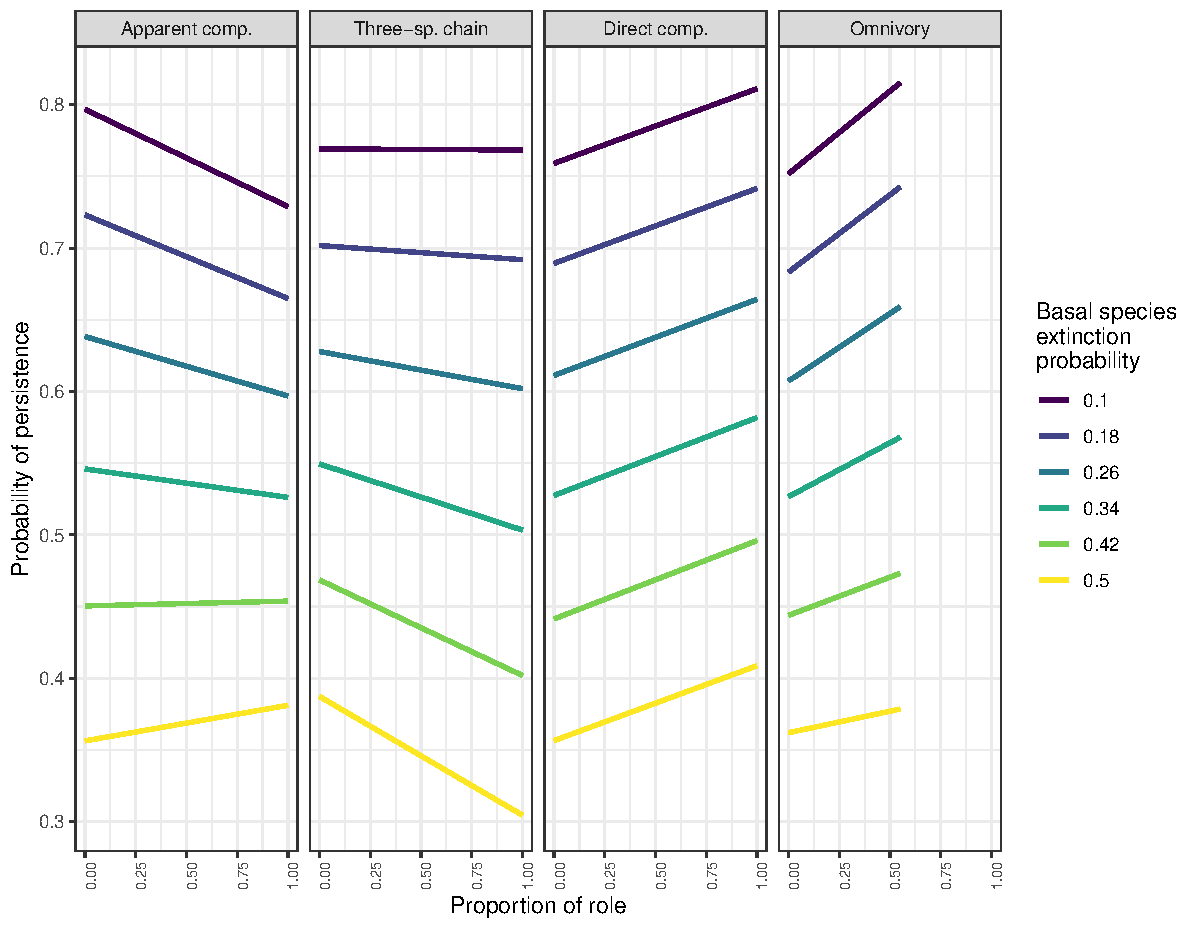
\includegraphics[width=\textwidth]{figures/prop_lmer_allCS.pdf}
                \caption{The effect of proportion of the role (x-axis) made up by various motifs (columns) on persistence (y-axis). The effect of participating in each motif was based on linear mixed-effect models following Equation~\ref{propreq}, except that models for each  disturbance level are fitted separately. The different colored lines indicate the probability of extinction of basal species, from $\pi_{disturbed} = 0.1$ (top, purple; no disturbance) to $\pi_{disturbed} = 0.5$ (bottom, yellow; high disturbance). Note that omnivory made up a smaller proportion of species' roles than other motifs; lines are plotted over the observed ranges of motif participation.}
                \label{fig:prop_lmer_all}
            \end{figure}
        
        \clearpage
    
        \subsubsection*{Consistency of  relationships across networks}
            
            When fitting regressions of persistence against motif participation for each network separately, networks with high connectance generally had more consistent relationships between persistence and motif participation, i.e., sharper peaks of the density distributions (Fig.~\ref{fig:density_prop_C}).
            However, this trend varied at different levels of disturbance, especially for the direct competition and omnivory motifs.
            At low and medium connectances there was little change in the distribution of slopes for direct competition across all levels of disturbance. 
            At high connectances, however, the proportion of positive slopes was both lower overall and decreased with increasing disturbance. 
            For the omnivory motif these trends were reversed. 
            Moreover, the omnivory motif has a particularly broad distribution of slopes (i.e., an inconsistent relationship to persistence) when network connectance was low. 
            Network size had a much smaller effect than connectance (Fig. S3; \emph{Appendix SE}).


        \begin{figure}[h!]
            \centering
            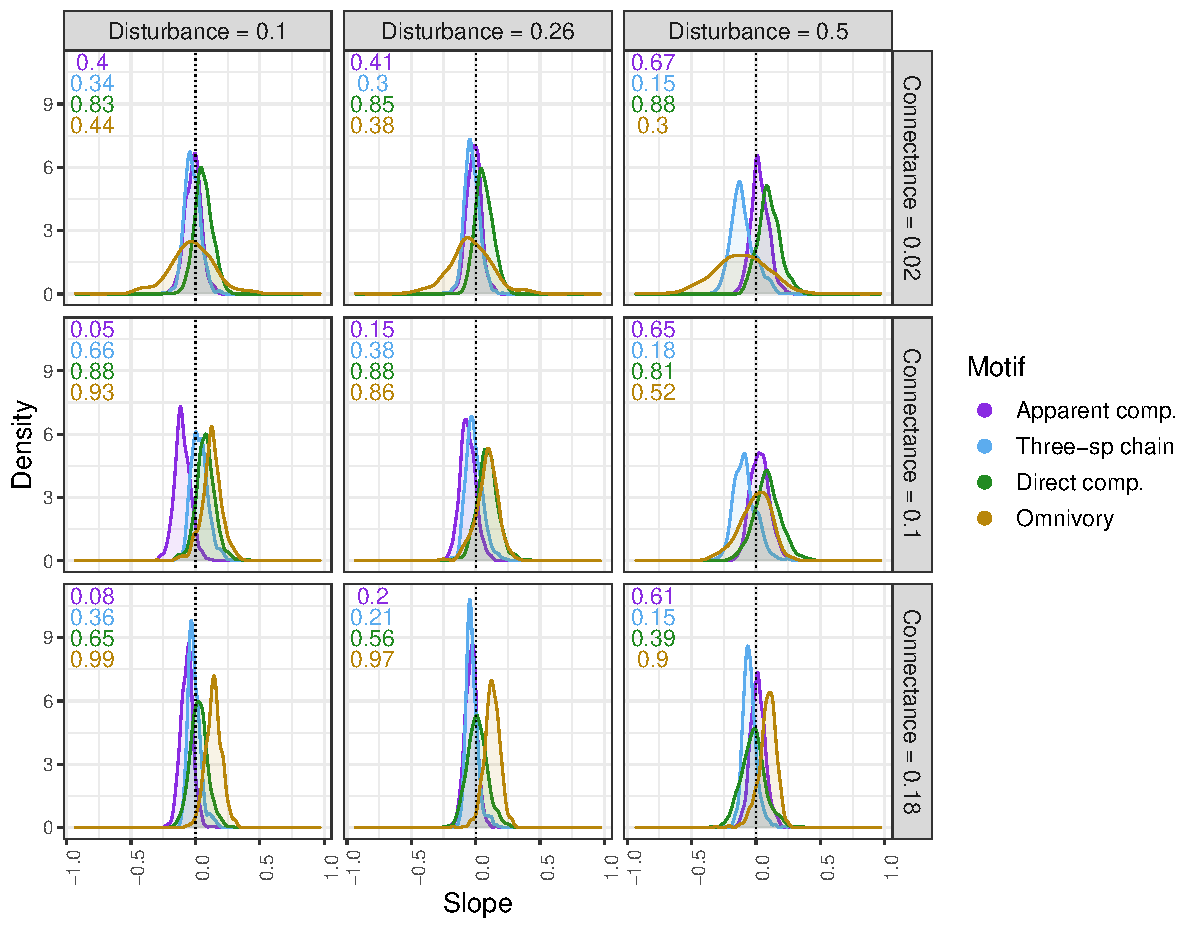
\includegraphics[width=\textwidth]{figures/prop_dens_bp_vs_C_allS.pdf}
            \caption{Here we show the density (y-axis) of slopes (x-axis) of persistence against proportion of different motifs for all simulated webs of all sizes - a visualization of how an increased proportion of each motif (different colored lines) affects persistence of consumer species. Columns show the result for various disturbances on the basal level, from $\pi_{disturbed} = 0.1$ (left) to $\pi_{disturbed} = 0.5$ (right). Rows show various levels of connectance. The dotted, vertical line indicate zero on the x-axis. A negative slope value reflects a negative relationship between increased participation in a motif and persistence, while a positive slope value reflects a positive relationship - an increased proportion of a specific motif increase persistence. The fraction of replicates with a slope greater than zero are stated in numbers in each sub-plot, the color corresponding to each motif (legend). }
            \label{fig:density_prop_C}
        \end{figure}    
    
    \subsection*{Species characteristics and persistence}
    
        Species persistence varied with both in-degree and trophic level (Fig.~\ref{fig:motifs_vs_TL_and_deg}; \emph{Appendix SF}). 
        Increased trophic level was generally associated with decreasing species persistence, although the rate of decline was slower at high disturbance (Table S5, \emph{Appendix SF}).
        In-degree showed an even stronger interaction with disturbance; having more prey species was associated with higher persistence without disturbance, but lower persistence at high levels of disturbance.


    
    \subsection*{Motif participation, network properties, and species characteristics}

        Species' motif participation varied depending on the properties of the network; size, connectance, and their interaction (Fig. S4, Table S6; \emph{Appendix SG}).
        Species appeared most often in the apparent competition motif in all types of networks, but the frequency decreased with increasing network size and connectance.
        The frequency with which species participated in the omnivory motif increased sharply with increasing connectance, while the frequency of the direct competition motif increased slightly with increasing network size. 
        
        Species' motif participation also varied with their in-degree and trophic level (Fig.~\ref{fig:motifs_vs_TL_and_deg}).
        Species with higher in-degree tended to have higher frequencies of participation in the omnivory motif. Proportions of the other three motifs tended to decline with increasing degree.
        Species with higher trophic levels tended to have higher proportions of apparent competition and three-species chains. 
        

            \begin{figure}[h!]
                \centering
                \includegraphics[width=.75\textwidth]{figures/roles_vs_TL.eps}
                \caption{As with motifs, persistence varied with simpler measures of species roles in networks. Moreover, motif frequencies correlated with in-degree and trophic level. \textbf{A-B)} Persistence increased with increasing in-degree for low levels of disturbance to basal resources but decreased with increasing degree for high levels of disturbance to basal resources.
                Persistence declined with inceasing STL for all levels of disturbance to basal resources.
                \textbf{C-D)} The proportion of omnivory increased with increasing degree while all other proportions decreased. The proportions of omnivory and direct competition decreased with increasing STL while the proportions of apparent competition and three-species chains increased.}
                \label{fig:motifs_vs_TL_and_deg}
            \end{figure}        
        


\clearpage

%Somewhere early in discussion (needs tidying up):
%Apparent comp and direct comp have no indirect effects in BN, so we should be able to explain them with simpler properties.


\section*{Discussion}


% Focus on what additional information is revealed from analyzing motif compared to global network properties or species characteristics.
% Connect to traits -- Cirtwill & Eklöf, 2018, Ecol Lett. 
% Bayesian network approach - what extra information does motifs provide when we are interested in bottom- up effects. 
% * Difference between 3-sp chain and omnivory, the importance of the rescue prey in omnivory (in dynamical sims omni was mostly bad, 3-sp chain good). Omni link destabilizing if strong, stabilizing if weak (other studies). In BN just a link as important as other links
% * Omnivory in fig 5 - high connectance, always good, not as good with lower levels of C
% * Extra prey in omnivory changes from being a security to a liability (with increasing disturbance?)
% * ADD REFS - high disturbance scenario is analogous to decreasing plant diversity


% Results summary - network level (following Anna)
    It has repeatedly been shown that global network properties are important for how well a network can handle disturbances such as loss of species \citep{Eklof2006, Dunne2002}. 
    At the same time, from a conservation perspective it is often more relevant to focus interventions on particular target species~\citep{}. 
    If target species are not selected \emph{a priori} based on economic or cultural concerns~\citep{}, then it is logical to target conservation efforts towards species that are most at risk of extinction.
    Identifying characteristics of a species' position within a network that are associated with increased or decreased persistence in the face of disturbance can assist with such efforts to direct scarce resources to the species which need them most.


    Motifs, the basic building blocks of networks~\citep{Milo2002}, are promising candidates for network structures that may be relevant to persistence.
    Motifs connect network-wide (global) and species-specific (local) properties, describing direct and indirect effects which can both affect network stability~\citep{} and species persistence~\citep{}. 
    As such, the distribution of three-species motifs is also related to network stability~\citep{}.
    We extend this previous research and show that both the distribution of motifs at the network level and the set of motifs a target species participates in are related to that species' persistence after disturbance to the plant community. 

    A network's motif profile had a relatively strong relationship to the network mean persistence compared to global structures (i.e., size and connectance). 
    However, connectance did affect which network motifs were most common. 
    For example, highly-connected networks tended to contain higher frequencies of the omnivory motif which includes more links than the other three-species motifs considered here.
    Thus, global-scale properties seem to have stronger effects on network persistence by changing meso-scale properties than directly.
    This in turn suggests that network motif profiles may be more useful than global network properties when predicting network-level mean extinction risk.

    % Network-level persistence
    In general, average persistence across a network was lowest in networks with high frequencies of the omnivory motif and highest in networks with high frequencies of the apparent competition motif. 
    Both of these motifs have been linked to stability of ecological networks.
    Apparent competition ...
    Omnivory has been proposed as both a stabilizing an destabilizing structure.
    When modelled in isolation, the omnivory motif is moderately likely to be stable while the other motifs we consider are highly likely to be stable~\citep{Borrelli2015a}.
    In empirical systems, higher levels of omnivory ...
    
    
    As expected based on the network-level effects, participation in the omnivory and apparent competition motifs was also strongly related to each species' probability of persistence.
    In contrast to the network-level results, participating more frequently in the omnivory motif \emph{increased} a species' probability of persistence with participating more frequently in the apparent competition motif \emph{decreased} persistence, except at very high levels of disturbance.
    These species-level trends may be explained by relationships between motif participation, in-degree, and trophic level.
    
    
    Participation in the apparent competition motif was strongly negatively correlated with in-degree and positively correlated with trophic level --a high proportion of the apparent competition motif implies a low in-degree and high trophic level, both of which are associated with lower probabilities of persistence.
    Moreover, the relationships between persistence and in-degree and apparent competition have a similar interaction with disturbance.
    Both are associated with lower persistence at low disturbance but increased persistence at high disturbance. 
    This may occur because, when disturbance is high, connections to many prey species mean many sources of bottom-up disturbance.
    - also strongly associated with trophic level but effects don't match. So there must be something else affecting the affect of apparent competition
    
    
    The omnivory motif showed opposite trends, being strongly and positively correlated with in-degree and negatively correlated with trophic level.
    A species with a high frequency of participation in the omnivory motif is therefore likely to have many prey and a low trophic level, both of which are associated with higher probabilities of persistence.
    The combination of low trophic level and high in-degree means that participating in the omnivory motif was positive at all levels of disturbance, while a high in-degree alone was not.
    This also demonstrates how motif participation can synthesize complementary information provided by other measures of species' positions within networks. 


    Discussion of the distribution results could go here...
 

% The effect of the local-scale network properties in-degree and trophic level differed.
% A high trophic level was associated with lower persistence across all levels of disturbance. This was expected, as species at higher trophic levels here by definition have equal or higher probability of extinction compared to their prey ~\citep{Eklof2013}.
% The effect of in-degree is less obvious and depended on the level of disturbance; a high in-degree had a positive effect on persistence at low levels of disturbance but not at high levels of disturbance.
% In addition to these different relationships with persistence, in-degree and trophic level had different relationships to the four motifs we investigated.




The direct competition motif was not strongly correlated to in-degree, but had a strong negative relationship with trophic level. Thus, species with a high proportion of the direct competition motif has in general a low trophic level, which is associated with higher probability of persistence at all levels of disturbance.
The clear positive relationship between proportion of the direct competition motif and species persistence is therefore likely due to the tendency for species at low trophic levels to have a higher proportion of that motif.


%The remaining two motifs are strongly related to both in-degree and trophic level and must be explained using a combination of the two simpler network properties.
%Motifs can, in this sense, act as a tool for synthesizing the information provided by multiple other measures of a species' place in its community, as well as interactions between them.
%The three-species chain motif, for example, is moderately negatively correlated with in-degree and moderately positively correlated with trophic level. 
%The relationship between persistence and the chain motif therefore combines the overall negative effect of high trophic level with the interaction between in-degree and disturbance; leading the chain motif to have little relationship to persistence at low disturbance and an increasingly negative relationship at higher disturbance.
Likewise, the three-species chain motif is correlated with trophic level, but the relationship is positive and a high proportion of this motif indicates a high trophic level. Hence, the negative effect on persistence of having a high proportion of the three-species chain motif is likely connected to the high trophic level. 
- sig. correlated with in-degree (I think???) but does not show up in the relationship to persistence
- something else is related to chain that acts like a positive association with in-degree that is strong enough to cancel out the negative relationship with in-degree



% % Might be able to add some of this paragraph to the one above or below (especially the refs).
% The divergent effect on persistence of either having a high proportion of the three-species chain or omnivory motif can, within our Bayesian Network framework, be explained by the structure of the food web.
% When participating in a food chain motif---three-species chain or omnivory---the top species of this structure will have a higher susceptibility since disturbances amplify through the network. In our results, this is in particular evident for the three-species chain motif at higher levels of disturbance, but this also applies to species with a high proportion of the omnivory motif. While the relationship between omnivory and persistence is strongly positive at low bottom-level disturbance, the trend is reduced at high levels of disturbance. 
% This is because species participating to a high extent in omnivory motifs share the sensitivity of species participating to a high extent in three-species chain motif, and are similarly negatively affected by bottom-level disturbances. However, the top species in an omnivory motif also have the benefit of an additional prey species, located further down in the food web. This prey item can assist as a buffer, decreasing the negative effect of disturbance on the consumer species. Clearly, this additional prey is of importance, since it is more beneficial with a higher proportion of the omnivory motif for an individual species than a high proportion of the three-species chain motif. 
% Thus, the observed benefit of a high proportion of the omnivory motif can be compared to omnivores in a network feeding adaptively. Studies have demonstrated that adaptive omnivory can increase the permanence of three-species chains \citep{Fagan1997, KrivanDiehl2005, AbramsFung2010}.
% Although species in our model cannot swap prey dependent on bottom-level disturbances or lower resource densities, a species with a high proportion of omnivory will in a sense spread its risk between prey items at different trophic levels.



%The relationship between omnivory and stability is subject to a longstanding debate in ecology. Omnivory has been shown to both stabilize and destabilize communities, and the impact is highly dependent on network context \citep{bascompte2005simple, Monteiro2016, Kratina2012}. 
%For example, omnivorous interactions may not be stable in isolation, but instead stabilized by interactions with other species when embedded in a larger food web \citep{Kratinaetal2012}. Additionally, the possibility of omnivores to feed adaptively from different trophic levels can spread the risks, for example when the prey level are disturbed \citep{Fagan1997}.

 \cite{Cirtwill2021_inprep} analysed how species time to extinction varied depending on their network profile. They found that a high proportion of the omnivory motif resulted in a shorter time to extinction, while the other three stable motifs were associated with longer times to extinction. However, the study by Cirtwill and Wootton used a different approach using a fully dynamic simulation model also including top-down effects. 
 
Our study of network and species motif profiles show that information on and synthesis of the global and local network structures can provide important information on which conservation actions that will most successfully preserve biodiversity in ecological networks. When affected by disturbance of plant community... 

- maybe end with a brief summary/discussion of the effect of disturbance: seem to see a "tipping point" in both degree and motifs.

    %In previous studies of the effect of omnivory motifs, the strength of the omnivorous link can potentially be important. If this link is strong, it is shown to be destabilizing (REF), while stabilizing if weaker (REF). In our Bayesian Network setting, this link is indistinguishable from any other link in the food web which partly may explain why omnivory results in increased persistence of consumer species. 

    
    
    % % We can move this to the SI or delete entirely.
    % Although we performed analysis of both the effect of the absolute counts of motifs and the normalized motif role on persistence, we here focus on the normalized motif role.
    % This is because, the consistency of the relationships between persistence and the number of times a species appears in any of the possible motifs suggests that the observed effects of non-normalized motif roles are actually due to degree.
    % Species with higher degrees will with high probability appear in more motifs than species with low degrees.
    % It is possible for a species with low degree (few direct interaction partners) to participate in many motifs if it interacts with high-degree species (thereby obtaining many indirect interaction partners), but such a situation is fairly unlikely.
    % Because of this overlap between degree and absolute numbers of motifs, and because degree shows a similar trend to the motif counts [[to be confirmed]], we recommend that researchers consider degree and/or normalized motifs rather than absolute motifs.
    % When we consider the proportion of a species' role made up by each motif, the influence of degree is largely removed.
    % Given the similarly high $R^2$ values between the models using proportions of motifs and absolute counts, it does not appear that we lose much explanatory power by removing degree. 
    % Therefore, our main analysis focus on the effect of the normalized motif role on persistence.
    



    

% [[When can motifs still be useful predictors and add insight?]]
%     Our results suggest that some motifs are associated with higher persistence than others but that this depends on the level of bottom-up disturbance to the food web.
%     Detailed tests of how motifs affect network stability and species persistence ideally require the ability to manipulate the motif structure of a network directly (i.e., obtaining many replicate networks with set numbers of each motif). 
%     Current methods of generating simulated ecological networks (e.g., the niche and cascade models) do not incorporate information on motifs.
%     Researchers interested in relationships between motif structure and persistence must therefore generate large numbers of networks and hope that they contain the necessary variety of motifs.
%     This shotgun approach to simulating different distributions of motifs within networks makes it difficult to investigate the precise effects of different numbers of, for example, the three-species chain motif, whether it occurs high or low in the network, and similar questions.
%     Fortunately, software is currently in development to allow researchers to simulate networks with particular motif profiles.
%     We heartily encourage researchers interested in the effects of motifs on persistence to adopt these new methods as they become available.



    

\section*{Glossary}

\begin{table}[h!]
\label{glossary}
\caption{Glossary of terms relating to motifs and Bayesian networks}

\begin{tabular}{l|l}
    Term & Definition \\
    \hline
    Motif &  \\
    Network profile & \\
    Motif participation & \\
    Motif role & \\
    Bayesian network & \\
    Network persistence & \\
    Species persistence & \\
    In-degree & \\
    Trophic level (STL) & \\
    Disturbance ($\pi_{disturbed}$) & Probability that a basal resource will go extinct when extra disturbance is added. \\
    Baseline extinction&  When no disturbance is applied, $\pi_{base}$=0.1.\\
\end{tabular}
\end{table}

% Notes on what expressions and words to use
% "probability of extinction" or "level of disturbance" for the different disturbace scenarios?


\bibliographystyle{ecollett} 
\bibliography{anna_bib_new} % Abbreviate journal titles.

\end{spacing}

\end{document}

